\chapter{\label{chapter:Moderator}The Moderator}

The core executive for GMAT is the Moderator.  The Moderator controls program flow, creating
components through the factory manager that are then managed in the configuration manager, and using
these components to model missions in a sandbox.  The Moderator creates the engine components,
manages those components when necessary, and controls the processes in GMAT's engine.  It
initializes the Sandbox prior to a run, and launches the run in the Sandbox.  In other words, the
Moderator is the central control element of GMAT, acting as the mediator between users and the
internal elements of the system.  This chapter explains how the Moderator accomplishes these tasks.

\section{Moderator Design Principles}

The Moderator is designed to enforce loose coupling between the elements of GMAT's engine.  It acts
as an intermediary between user inputs passed in through the script and GUI interpreters, the
factory subsystem used to build objects needed to simulate a mission, the configuration that stores
these configured objects, and the sandboxes that actually run the simulation.

\begin{figure}[htb]
\begin{center}
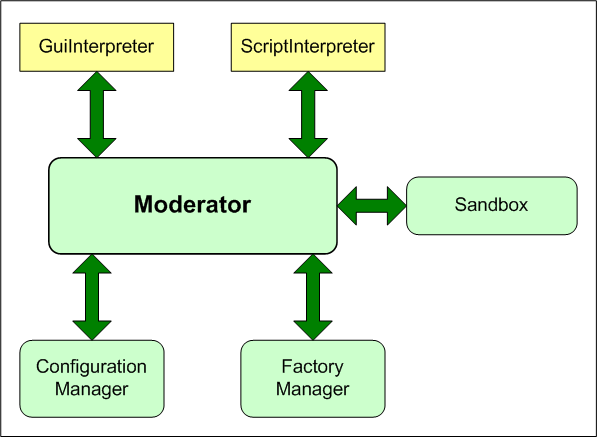
\includegraphics[239,175]{Images/ModeratorInteractions.png}
\caption{Program Flow and the Moderator}
\label{figure:ModeratorInteractions}
\end{center}
\end{figure}

Figure~\ref{figure:ModeratorInteractions} shows the connections between the Moderator and the other
management components of the GMAT engine.  All communications between these elements of the system
are shown in the figure, illustating the central role of the Moderator in GMAT.

Chapter~\ref{chapter:TopLevel} provided several illustrative examples of how GMAT performs typical
tasks required to run a mission.  The following paragraphs describe the key interactions between the
Moderator the other components shown in Figure~\ref{figure:ModeratorInteractions}.  The class
design for the Moderator is derived from these interactions, and is explained in the next section
of this chapter.

\subsection{Object Creation}

Users specify the objects that they need in their simulation using either GMAT's scripting language
or the graphical user interface (GUI).  There are two types of objects that are created this way:
resources, which are objects that are used in various ways in the timeline of the simulation, and
commands, which constitute the user's design of the mission timeline.  The resources are created by
lines in a script that start with the keyword ``Create'', or by selecting the ``Create'' options on
the GUI's resource tree.  Commands are created on GMAT's mission tree using the ``Insert...'' and
``Append'' commands from the GUI, or through typing the commands in time order in the script.

\begin{figure}[htb]
\begin{center}
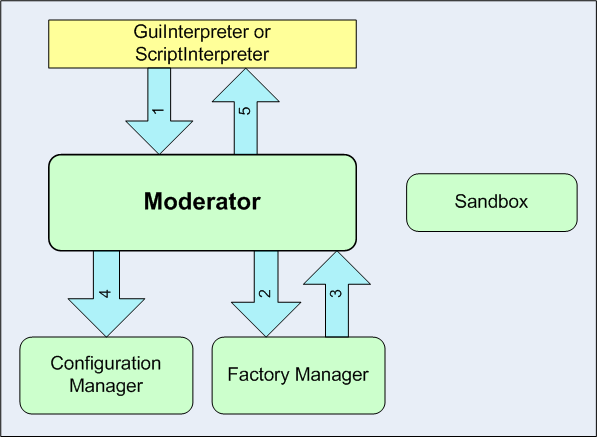
\includegraphics[239,175]{Images/ModeratorCreate.png}
\caption{Program Flow and the Moderator}
\label{figure:ModeratorCreate}
\end{center}
\end{figure}

Figure~\ref{figure:ModeratorCreate} shows the object creation process from the Moderator's
viewpoint.  The information flow through the Moderator proceeds in 5 steps:

\begin{enumerate}
\item The process starts with a creation action taken by a user.  This action generates a message
requesting the creation of the object.  The message is passed to the either the script or GUI
interpreter, which then sends the message to the Moderator.
\item The creation message contains the type of the object that needs to be created, along with the
name of the object and, in some cases, additional parameter data.  The Moderator passes these data
to the factory manager.
\item The factory manager manages the object creation, and returns either a pointer to the created
object or a NULL pointer to the Moderator.
\item If an object was created, the Moderator passes its pointer to the configuration manager if the
object is a resource, or the mission control sequence if the object is a command.
\item The object pointer is returned to the interpreter.
\end{enumerate}

\subsection{Object Configuration}



\subsection{Mission Initialization}



\subsection{Mission Execution}



\subsection{Data Persistance}



\section{Moderator Design}

\begin{figure}[htb]
\begin{center}
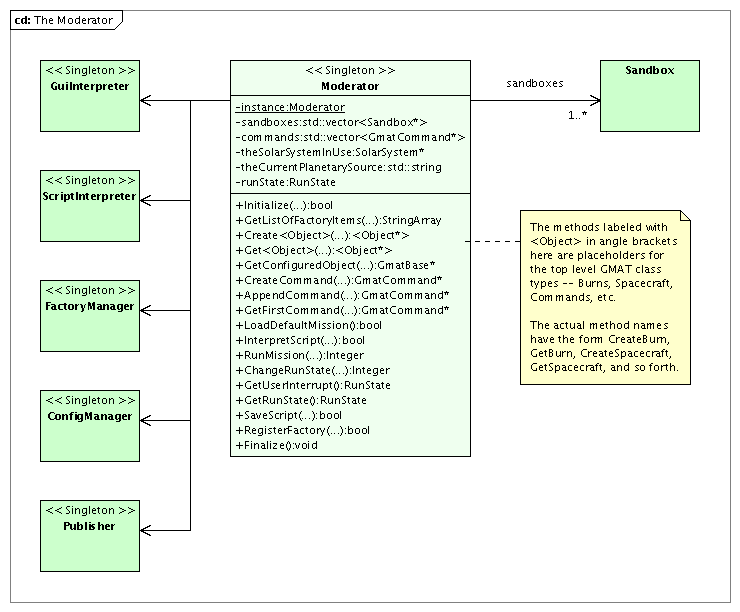
\includegraphics[370,346]{Images/TheModerator.png}
\caption{The Moderator in its Environment}
\label{figure:ModeratorClassDiagram}
\end{center}
\end{figure}

Figure ~\ref{figure:ModeratorClassDiagram} shows the Moderator, the classes it interacts with, and
some of its internal structures.  The interactions between the Moderator and other elements of
GMAT's engine were presented in Chapter~\ref{chapter:TopLevel}.  The sequence diagrams presented
there describe at a high level the interfaces to the Moderator and their usage when constructing a
model.  The methods shown in Figure~\ref{figure:ModeratorClassDiagram} present these interfaces in
more detail.  The following paragraphs describe these interfaces and the internal data members used
by the Moderator.




Important Data Structures

Important Interfaces

Coupling and component relationships

Which methods are likely to be used and called directly, and which are called via other interfaces


\section{\label{section:ModeratorStates}States Transitions in the Moderator}

The Moderator tracks the current state of the system using a parameter named runState, which is set
to a value in the RunState enumeration (see Table~\ref{table:RunStateEnum}) defined in the Gmat
namespace.  The engine states tracked in the Moderator are the IDLE, RUNNING, and PAUSED states.
The transitions

\begin{figure}[htb]
\begin{center}
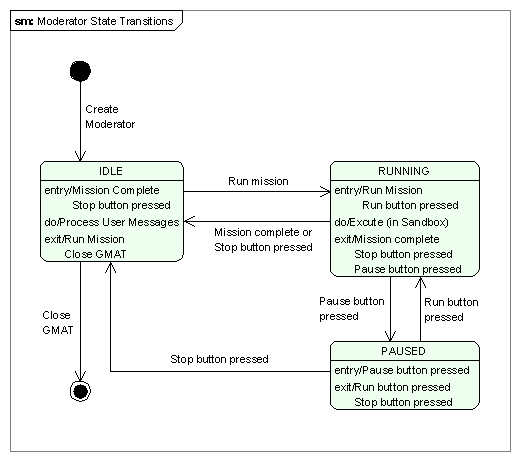
\includegraphics[260,231]{Images/ModeratorStateTransitions.png}
\caption{State Transitions in the Moderator}
\label{figure:ModeratorStateTransitions}
\end{center}
\end{figure}

Figure ~\ref{figure:ModeratorStateTransitions} shows the run state transitions tracked by the
Moderator.  The Moderator is created with the run state set to the IDLE state.  Most of the time,
the Moderator remains in the IDLE state, processing messages from users and managing the internal
components of the GMAT engine\footnote{Many of the activities performed by the Moderator in the IDLE
state are described in Chapter~\ref{chapter:TopLevel}.  Additional Moderator interactions with the
other engine components are described in the appropriate sections of this document.}.

When a user executes a Mission Control Sequence, the Moderator transitions to the RUNNING state.  In
this state, the Moderator performs very limited processing while the control of the system is
managed by the sandbox that is running the mission.  The sandbox polls the Moderator for user
activity at convenient points during the mission run.  This polling allows the Moderator to respond
to user actions that either terminate the mission early or pause the mission.

If the user presses the pause button on the GUI, the Moderator transitions into the PAUSED state
when the sandbox polls for state status.  This activity stops the mission run, but maintains data so
that the run can be resumed from the point of the stop.  The user tells the Moderator to resume the
run by pressing the run button on the GUI.  When the Moderator receives the run message, it
transitions back into the RUNNING state and tells the sandbox to resume the run.

The user can terminate a run early by pressing the stop button on the GUI during a run.  This action
always causes the Moderator to transition from its current state - either RUNNING or PAUSED -- into
the IDLE state.


Sequence or activity diagrams for basic operations (if appropriate)


\section{Best Practices}

When should you modify the Moderator

Best Practices and Philosophy
